\documentclass{scrartcl}
\usepackage{mm_ws15}

\newcommand{\sheetTitle}{Blatt 11, Abgabe 19.1.2016}
\renewcommand{\ee}{\vec{e}}
\begin{document}
\maketitle


%%%%%%%%%%%%%%%%%%%%%%%%%%%%%%%%%%%%%%%%%%%%%%%%%%%%%%%%%%%%%%%%%%%%%%%%%%%%%%%%
\section{Kurven und Kurvenlängen}
\label{sec:kurven_und_kurvenl_ngen}

Finden Sie für die folgenden Kurven im $\RR^2$ von $(0,0)$ nach $(2,0)$ geeignete Parametrisierungen:
\begin{align*}
  \mathbf{A}&\colon (0,0) \to (0,1) \to (2,1) \to (2,0) \quad& \mbox{auf drei geraden Teilkurven} \\
  \mathbf{B}&\colon (0,0) \to (1,1) \to (2,0) \quad& \mbox{auf zwei geraden Teilkurven} \\
  \mathbf{C}&\colon (0,0) \to (2,0)  \quad& \mbox{auf einem Halbkreisbogen}
\end{align*}
Berechnen Sie anschließend die Bogenlängen der drei Kurven über das Linienintegral $L(\gamma) = \int_\gamma \dd r$.

\begin{center}
  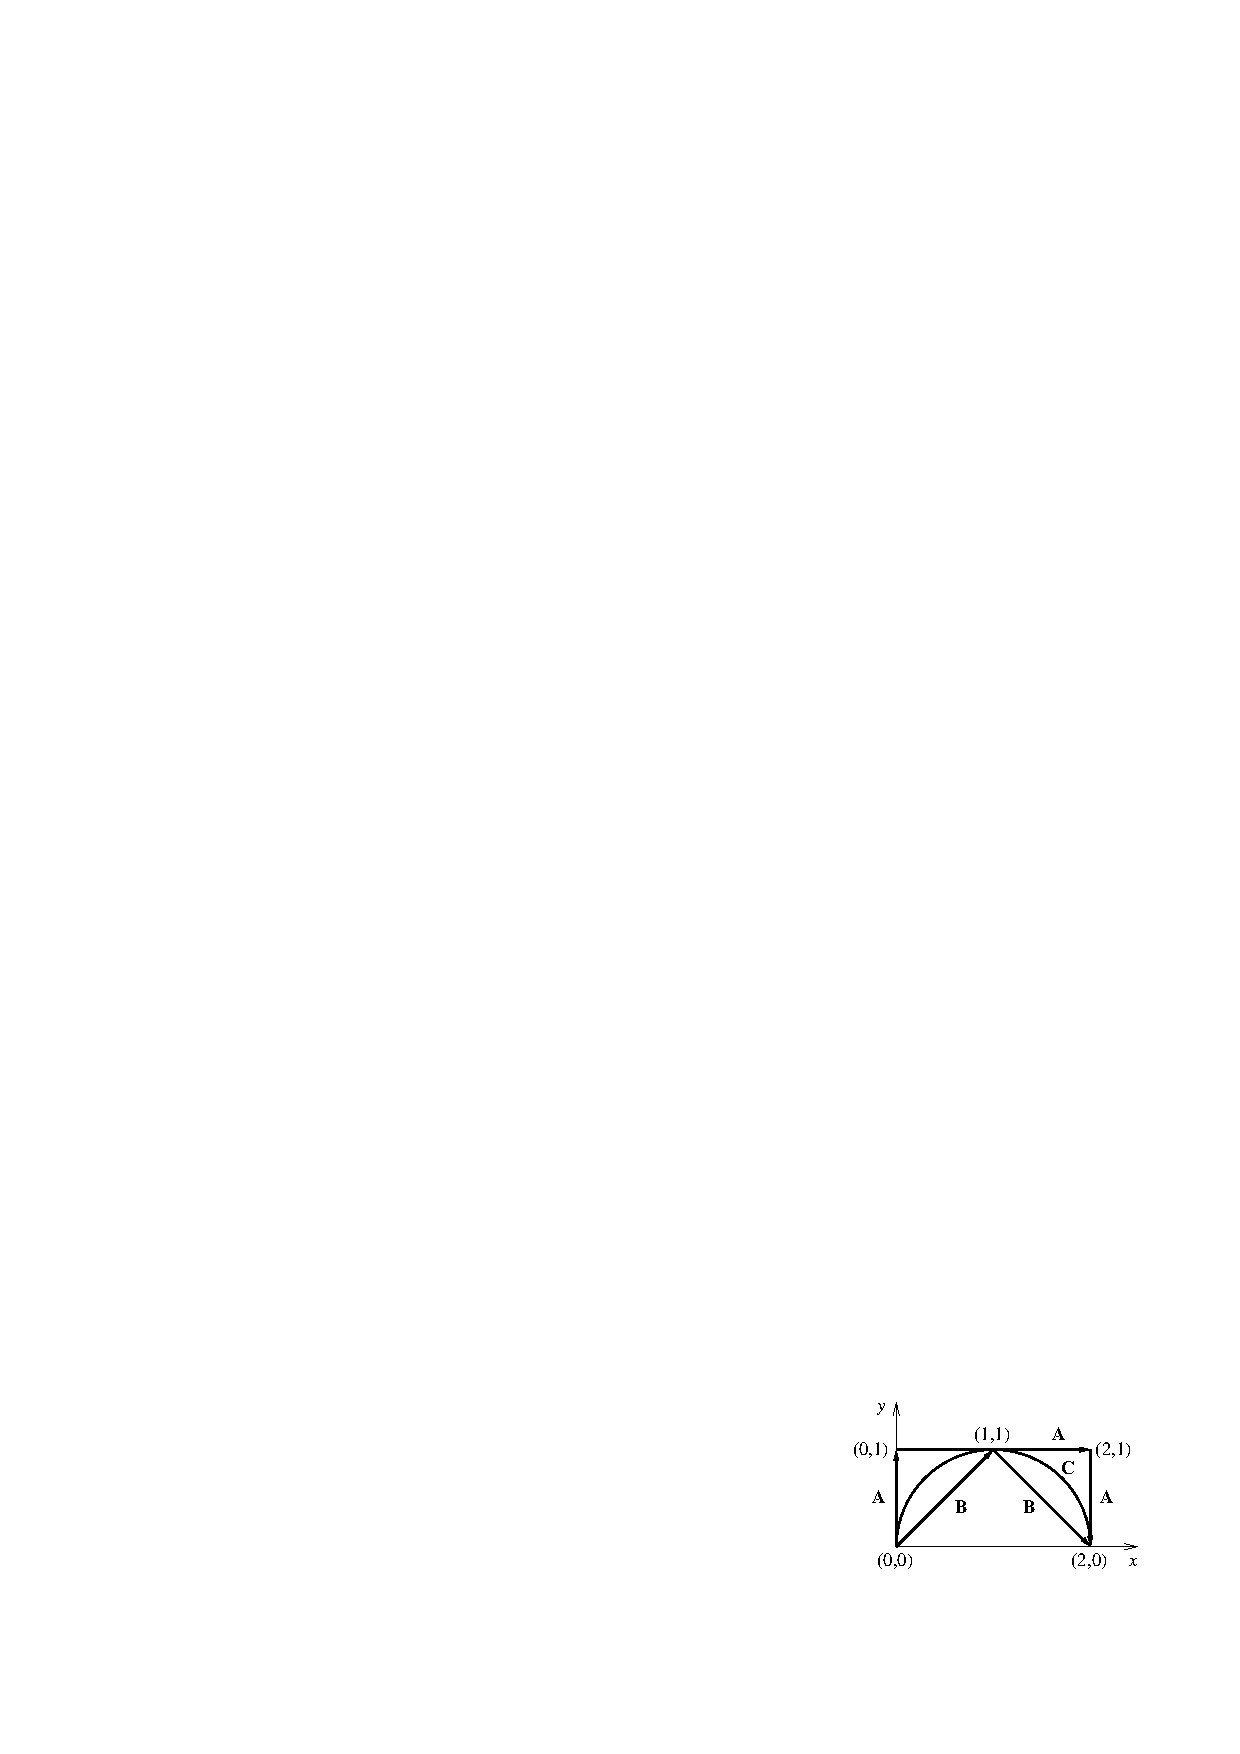
\includegraphics[width=.5\textwidth]{img/curves}
\end{center}

%%%%%%%%%%%%%%%%%%%%%%%%%%%%%%%%%%%%%%%%%%%%%%%%%%%%%%%%%%%%%%%%%%%%%%%%%%%%%%%%
\section{Länge der Brachistochrone}
\label{sec:bachistochrone}

Die Kurve, auf der ein Massenpunkt die Strecke zwischen zwei Orten $\vec x_1$ und $\vec x_2$ in einem Schwerefeld ohne Reibung am schnellsten zurücklegt nennt man die Brachistochrone.
(Johann Bernoulli stellte diese Aufgabe 1696, obwohl er die Lösung schon zuvor gefunden hatte. 
Ein Jahr später wurden seine und vier weitere Lösungen veröffentlicht, u.a.\ von Johanns Bruder Jakob sowie Isaac Newton und Gottfried Leibniz. 
Diese Arbeiten gelten als Geburtsstunde der Variationsrechnung.)
Die Brachistochrone für die Punkte $\vec x_1 = \colvec{0 \\ 0}$ und $\vec x_2 = \colvec{0 \\ 2 \pi R}$ kann man wie folgt parametrisieren:
\[
  \vec{\varphi}\colon [0, 2\pi] \to \RR^2, \, t \mapsto \vec\varphi(t) = \colvec{R (t - \sin t) \\ R (\cos t - 1)}.
\]
Skizzieren Sie die Kurve und zeigen Sie dass die Länge $8R$ beträgt. 
Geben Sie eine Parametrisierung für den kürzesten Weg zwischen $\vec x_1$ und $\vec x_2$ an und berechnen Sie dessen Länge.
\begin{remark}{Hinweis}
  Der kürzeste Weg zwischen zwei Punkten im euklidischen Raum ist die Strecke zwischen ihnen.
\end{remark}


%%%%%%%%%%%%%%%%%%%%%%%%%%%%%%%%%%%%%%%%%%%%%%%%%%%%%%%%%%%%%%%%%%%%%%%%%%%%%%%%
\section{Linienintegrale: Arbeit entlang eines Weges}
\label{sec:linienintegrale_arbeit_entlang_eines_weges}

Ein Massepunkt der Masse $m$ bewegt sich in der Nähe der Erdoberfläche unter Einfluss der Gewichtskraft $\vec F_\mathrm{G} = - m g \ee_y$ entlang der Parabelbahn
\[
  \vec r(t) = t \ee_x + \left( -\frac{1}{2} t^2 + t \right) \ee_y
\]
mit $t \in [0,2]$.
\begin{subex}
  \item Skizzieren Sie die Bahnkurve $\mathcal{D} = \{ \vec r(t) | t \in [0,2] \}$ sowie das Kraftfeld $F_\mathrm{G}$.
  Berechnen Sie die für diese Bewegung aufzubringende Arbeit $W = - \int_\mathcal{D} \dd \vec r \dot \vec F(\vec r)$.
  \item Aufgrund eines Gegenwindes in $x$-Richtung wirkt \emph{zusätzlich} die Kraft $\vec F_\mathrm{W} = - c \ee_x$. Welche Arbeit muss nun aufgebracht werden?
\end{subex}


%%%%%%%%%%%%%%%%%%%%%%%%%%%%%%%%%%%%%%%%%%%%%%%%%%%%%%%%%%%%%%%%%%%%%%%%%%%%%%%%
\section{Linienintegrale: Wegunabhängigkeit}
\label{sec:linienintegrale_wegunabh_ngigkeit}

Betrachte die zwei Vektorfelder in $\RR^2$
\[
  \vec F_1(x, y) = \colvec{4x + xy \\ \frac{x^2}{2}} \quad \mbox{und} \quad \vec F_2 (x, y) = \colvec{4x + xy \\ x^2}.
\]
\begin{subex}
  \item Betrachte die folgenden beiden Wege von $(0,0)$ nach $(1,2)$ (siehe auch untenstehende Skizze):
  $\gamma_1$ sei die Strecke zwischen den beiden Punkten und $\gamma_2$ der Parabelast, der durch die beiden Punkte verläuft, sowie in $(0,0)$ sein Minimum annimmt.
  Finden Sie jeweils eine geeignete Parametrisierung $\gamma_i(t)$.
  \item Berechnen Sie das Wegintegral über $\vec F_1$ $\int_\gamma \dd \vec r \dot \vec F_1(\vec r)$ für $\Gamma_1$ und $\Gamma_2$.
  Nutzen Sie jeweils die Parametrisierung aus a).
  \item Berechnen Sie nun die Wegintegrale über $\Gamma_1$ und $\Gamma_2$ für das Vektorfeld $\vec F_2$.
\end{subex}

\begin{center}
  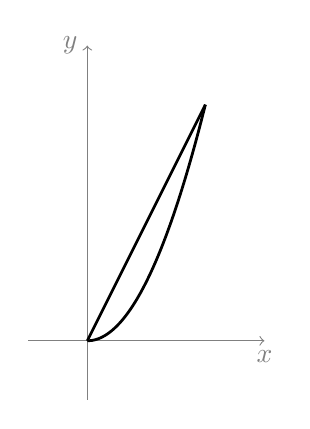
\begin{tikzpicture}[scale=1.5]
    \draw[gray,->] (-0.5,0) -- (1.5,0) node[below] {$x$};
    \draw[gray,->] (0,-0.5) -- (0,2.5) node[left] {$y$};
    \draw[domain=0:1,smooth,variable=\x,line width=1] 
      plot ({\x} , {2*\x});
    \draw[domain=0:1,smooth,variable=\x,line width=1] 
      plot ({\x} , {2*\x*\x});
  \end{tikzpicture}
\end{center}
\todo{Labels \& Endpoints}

\end{document}
